\section{Electroweak probes}
\label{sect:pas:ew}
%- Utility of penetrating probes
%- ALICE low pT photons measuring QCD temperature (cf. PHENIX)
%- Expected scaling of hard probes in A+B (nuclear thickness)
%- PDFs and nPDFs, calculation schemes (LO vs. NLO), codes
%- Z bosons (CMS first result cf. QCD), ATLAS Z centrality & rapidity
%- W (CMS published - can i compare to ATLAS prelim on a plot?)
%- Photon (CMS 2010, ATLAS prelim 2011?)

While a primary topic in the study of heavy ion collisions is the modification
of jets in the hot and dense nuclear medium, typical analyses of
hard processes have assumed that the
structure of a nucleon in a nucleus-nucleus collision is quantitatively the
same as one in a nucleon-nucleon collision.
From analyses of lepton-nucleus deep inelastic scattering data,
it is known that cross sections do not scale linearly with the number of nucleons,
as might be expected simply from the availability of scattering centers.
The deviations from this scaling are referred to generally as ``nuclear shadowing'',
and are typically shown as a function of Bjorken $x$ for different ranges in the
hardness scale $Q^2$.
The region around $x \sim 0.1$ corresponds to the valence quark region for a standard
nucleon, and this is usually enhanced.  The region above this, $x \geq 0.2$ is typically
suppressed (the so-called ``EMC effect''), while the region below $x << 0.1$ is also
suppressed down to very small values of $x$.  The latter phenomenon is more
typically known as ``nuclear shadowing'' and is thought to arise generally from
quantum mechanical effects which deplete the numbers with small fractions of the
nucleon momentum.

It is important to understand the magnitude of these sorts of effects in
the realistic environment of a heavy ion collision, in order to properly interpret
measurements of hard process rates relative to a nucleon-nucleon reference system.
At the RHIC collider, this was addressed early in the experimental program
through measurements of high $\pT$ particles in deuteron-gold collisions.
Presumably, any gross effects related to modifications of nucleon structure in the
nuclear environment would show up as modifications in this system.  It was found that
hadrons above $\sim 2$~GeV were produced at expected rates near $\eta =0$, confirming that
the high $\pT$ suppression observed in the early days of the RHIC program did not
arise from changes in nucleon structure, and strengthening the case for jet suppression
in the hot and dense medium.
However, it was also found that hadrons and J$/\psi$ particles were suppressed at
forward angles, in the direction of the incoming deuteron, especially in more ``central''
d+Au collisions, and enhanced slightly at backwards angles, in the direction of the
nucleus.  These features are in broad agreement with predictions from calculations
incorporating the nuclear shadowing observed in lepton-nucleus DIS.

While the measurement of hadronic final states in proton (or deuteron)--nucleus collisions
is thought to give useful information on modifications in the initial state of these
simpler systems, the above-mentioned observed modifications of jets precludes similar
observables giving similar information in heavy ion collisions.
For this reason, great attention has been given to the measurement of
``penetrating probes'', particles which do not interact strongly after they are produced.
While charged leptons and neutral photons, of course,
do not interact strongly, they come predominantly from
jets and hadrons at relative low $\pT < 20$~GeV.
However, at high $\pT$, most leptons are known to arise from the decay of electroweak
bosons (Z and W particles).  Furthermore, isolated photons at high $\pT$ are predominantly
``prompt'', i.e. arising from the direct interactions of quarks and gluons and not from
electromagnetic decays of hadrons ($\pi^0$ and $\eta$).

While the production cross sections for the heavy bosons are prohibitively small at the
top RHIC energies (200~GeV per nucleon-nucleon collision), the LHC provides the first
heavy ion system where all of the electroweak bosons are produced at substantial rates.
This section presents measurements of all three particles in \PbPb collisions at the LHC,
and shows their comparisons either with nucleon-nucleon reference data, or cross sections
calculated with perturbative QCD using standard structure functions.
The main physics goals of these measurements are twofold
\begin{itemize}
\item To establish whether the production of the vector bosons is proportional to the
nuclear thickness or, equivalently, the number of binary nucleon-nucleon collisions
\item To see whether any modifications of vector boson production can be observed,
and if they can be attributed to modifications of the nuclear PDFs
\end{itemize}
Theoretical calculations provide some guidance as to the magnitude of the modifications
of standard PDFs expected in nPDFs, but substantial uncertainties remain due to the
different parameterizations of the existing nDIS data.
One feature which is predicted generically, however, is the decreasing magnitude of
nuclear modifications with increasing $Q^2$.  As shown in Fig., the large magnitude
of shadowing expected at low $Q^2$ (i.e. low \pT) is reduced substantially even by
$Q^2=100$~GeV.  Thus, the large values of $M_{\mathrm Z}$ and $M_{\mathrm W}$ are already 80-90~GeV, naturally lead
to nuclear modifications only at the 10-15\% level.

\begin{figure}[t]
\begin{center}
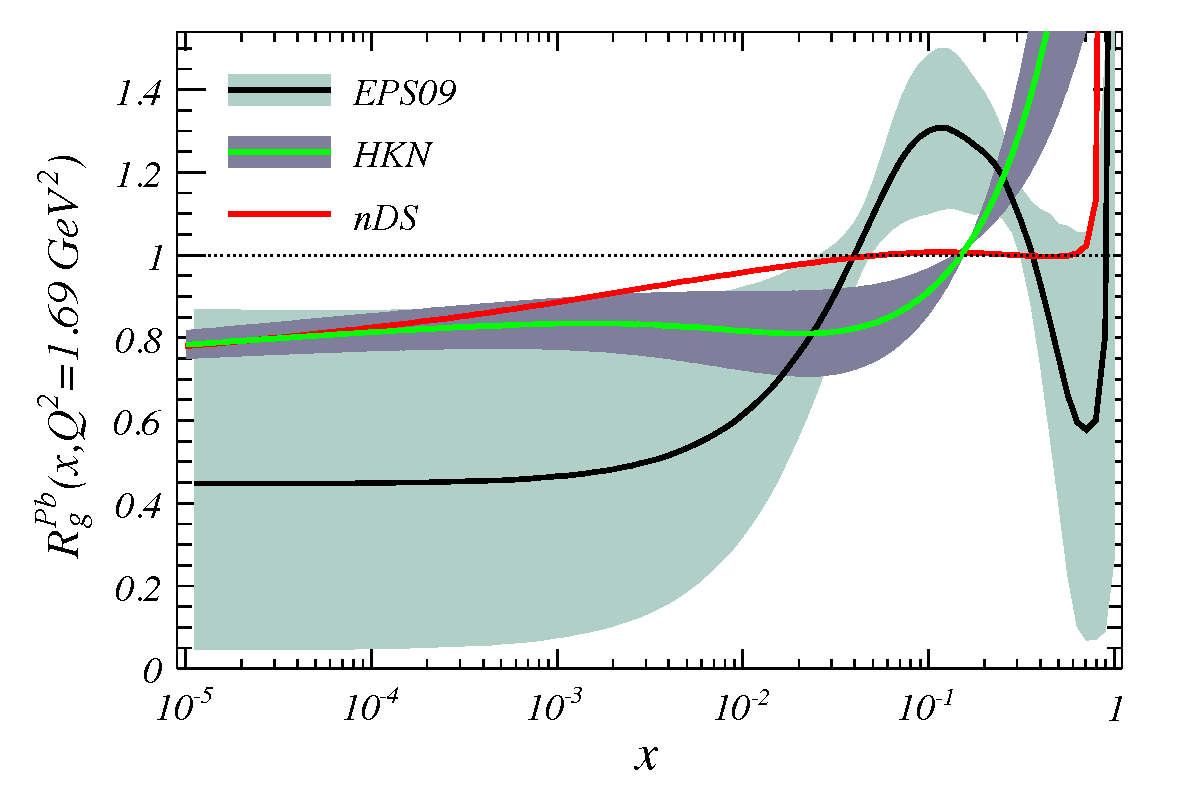
\includegraphics[width=0.49\textwidth]{electroweak_figs/gluonsnew.pdf}
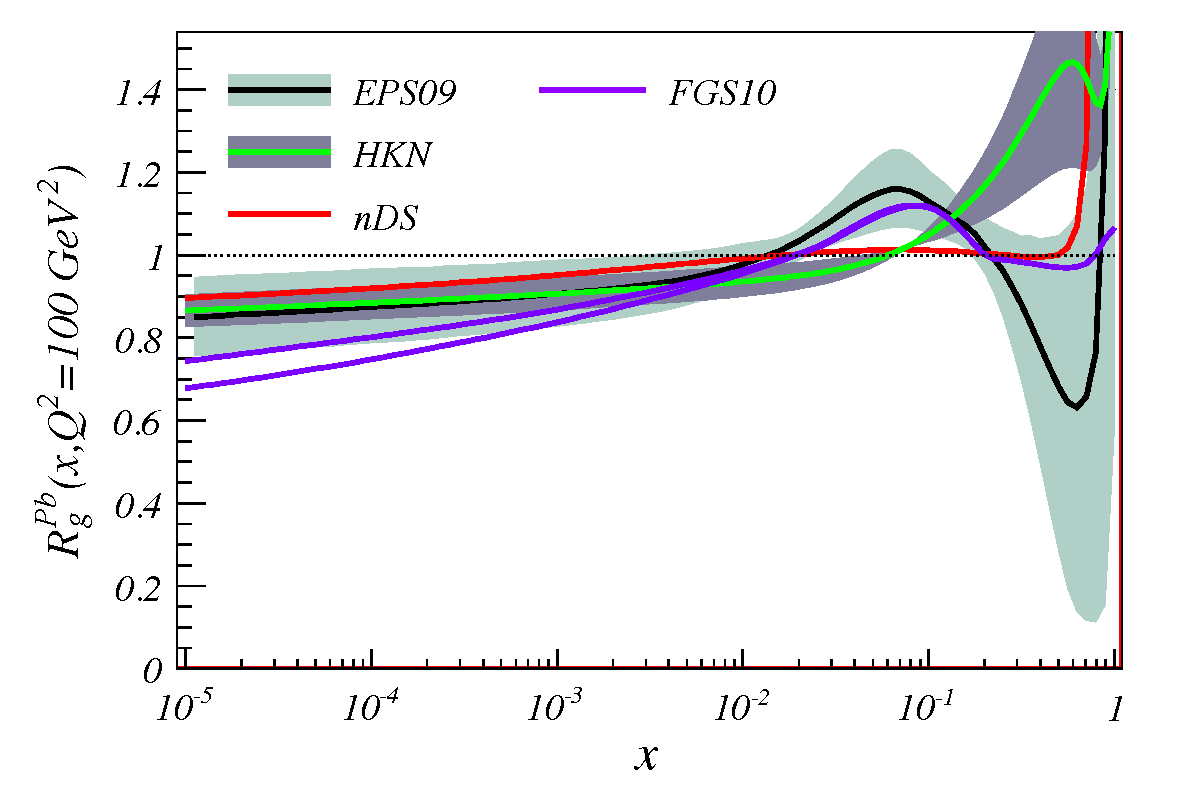
\includegraphics[width=0.49\textwidth]{electroweak_figs/gluonsnew100.pdf}
\caption[]{
(left) Modifications to proton PDFs expected from different nPDF implementations, for $Q^2=1.69$~GeV$^2$,
(right) Modifications to proton PDFs expected from different nPDF implementations, for $Q^2=100$~GeV$^2$.
From Ref.~\cite{Salgado:2011wc}.
}
\label{fig:pas:salgado}
\end{center}
\end{figure}

\subsection{Measurements of W and Z bosons in \PbPb\ collisions}

The first observation of vector bosons in \PbPb collision was performed by the ATLAS
experiment with a set of 38 Z candidates obtained in the first heavy ion run in 2010, which
was followed several months later by a CMS result comparing with theoretical calculations.
However, the statistical power of the 2010 sample was not sufficient to make strong conclusions
about the Z production rates as a function of the nuclear thickness.
The situation has improved dramatically with a published measurement of W bosons by CMS, also from the
2010 dataset, but benefiting from the large increase in the W cross section compared with Z.
ATLAS has also published the yield and spectrum of Z bosons from the much larger 2011 \PbPb dataset.
Together these give a relatively complete first look at the behavior of heavy vector bosons in
heavy ion collisions.


\begin{figure}[t]
\begin{center}
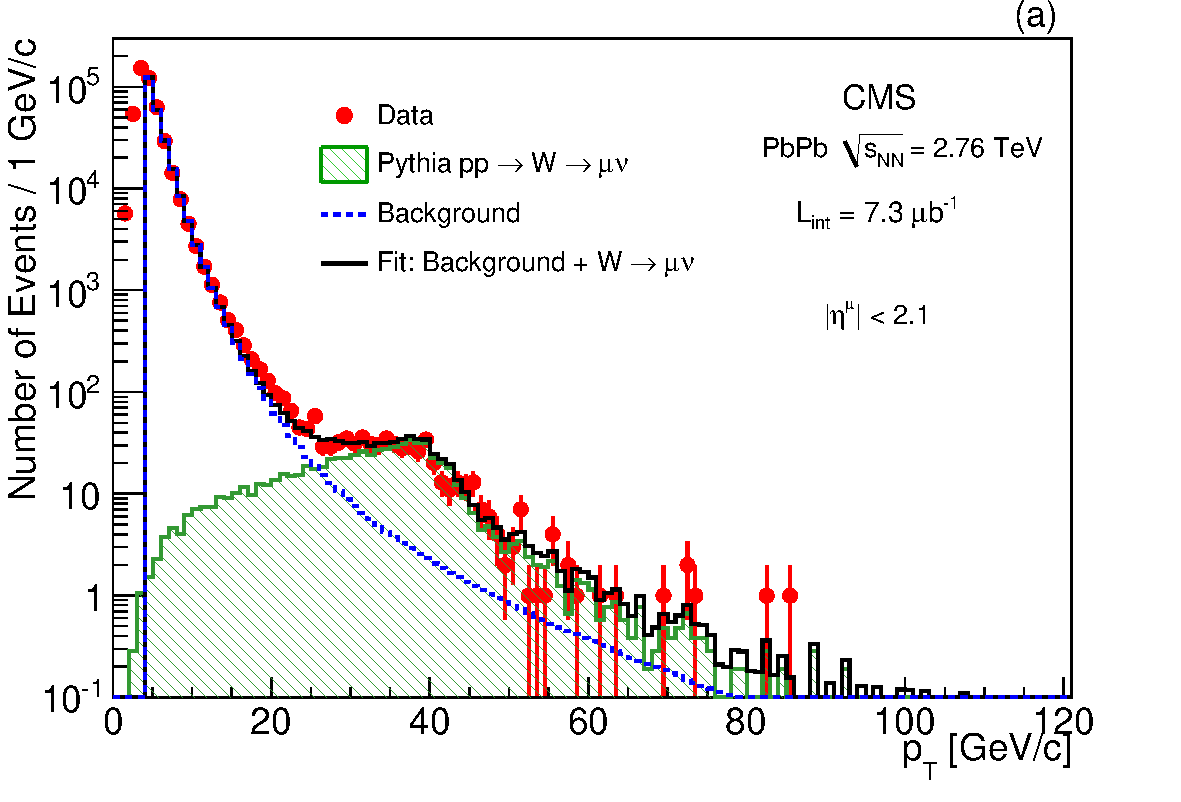
\includegraphics[width=0.49\textwidth]{electroweak_figs/Fig1a.pdf}
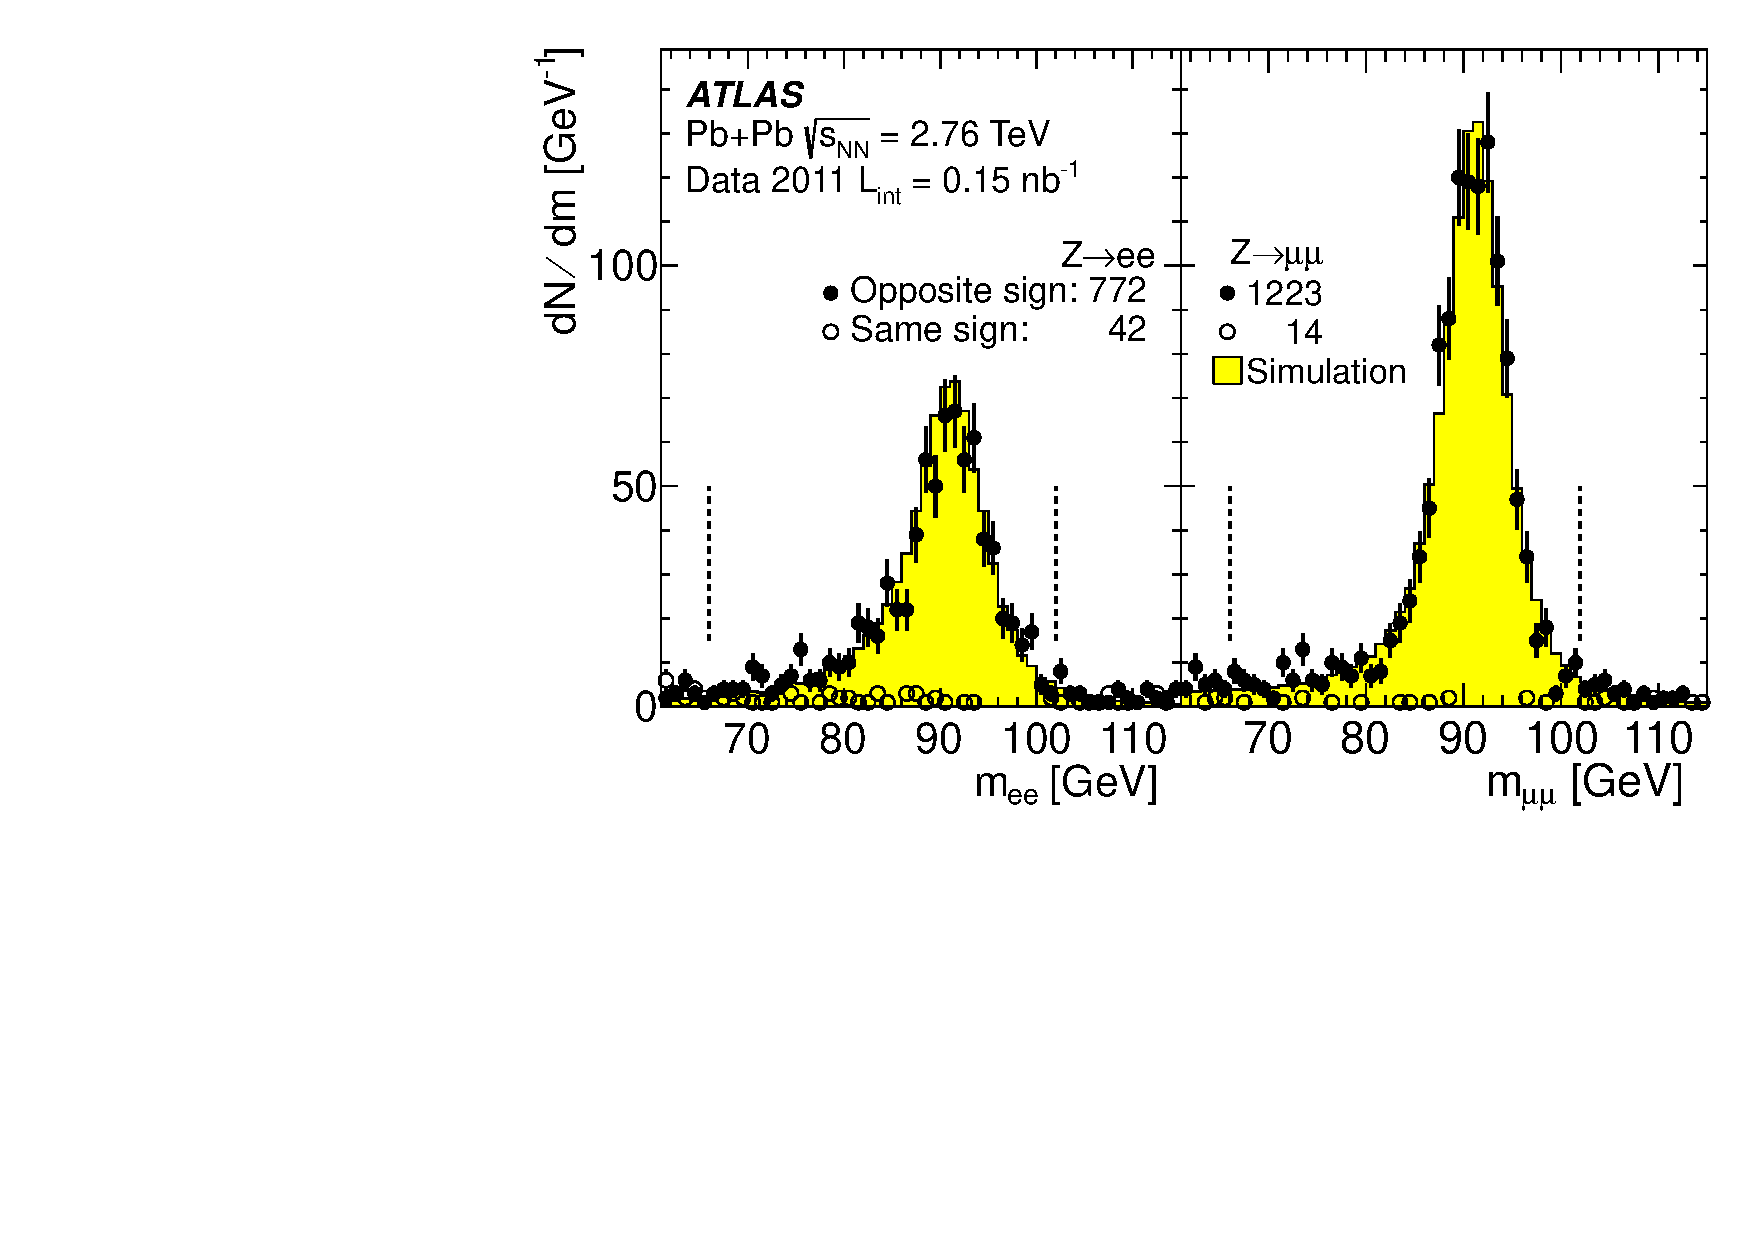
\includegraphics[width=0.49\textwidth]{electroweak_figs/fig_01.pdf}
\caption[]{(left) Single muon spectrum, after selection cuts, from CMS data~\cite{Chatrchyan:2012nt} (right) Dimuon mass spectrum, in electron and muon channels from ATLAS data~\cite{Aad:2012ew}.}
\label{fig:pas:zw_signal}
\end{center}
\end{figure}
The CMS W measurement was performed using the CMS inner tracker, which covers $|\eta|<2.4$
and the CMS muon spectrometer, which covers $|\eta|<2.4$ using a variety of gaseous detectors
(CSC, DT, with RPCs used for triggering), but was restricted to $|\eta|<2.1$ in this particular analysis.
The ATLAS Z measurement was performed combining dilepton decays in the muon and electron channels.
The ATLAS muon spectrometer uses drift tubes and cathode strip chambers to measure muons with $|\eta|<2.7$
in tandem with the ATLAS inner detector covering $|\eta|<2.5$.
Electrons are measured in ATLAS using the inner detector in association with the ATLAS calorimeter system,
which is particularly finely segmented in $\eta$ for $|\eta|<2.5$, allowing rejection of jet backgrounds.

As shown in Figure~\ref{fig:pas:zw_signal}(left) from CMS, the single muon spectrum at high $\pT$ clearly shows a contribution
from W bosons as a peak near 40~GeV.
The backgrounds from jets are strongly reduced by calculating the missing $\pT$ for each event with a
high \pT muon, based on tracks with $\pT>3$~GeV.  The background from Z bosons is removed by removing muons which
combine with a second muon in the same event that reconstructs to a mass near the Z mass.
After selections, about 540 W candidates were found in the 2010 \PbPb data.
%
Figure~\ref{fig:pas:zw_signal}(right) shows the dimuon and dielectron mass spectrum after requiring $\pT>10$~GeV for
the muons, and $\pT>20$~GeV for the electrons.  The Z lineshape is in good agreement with simulations for both
dielectron and dimuon channels.
After selections, about 2000 Z candidates were reconstructed in the 2011 \PbPb data.

\begin{figure}[t]
\begin{center}
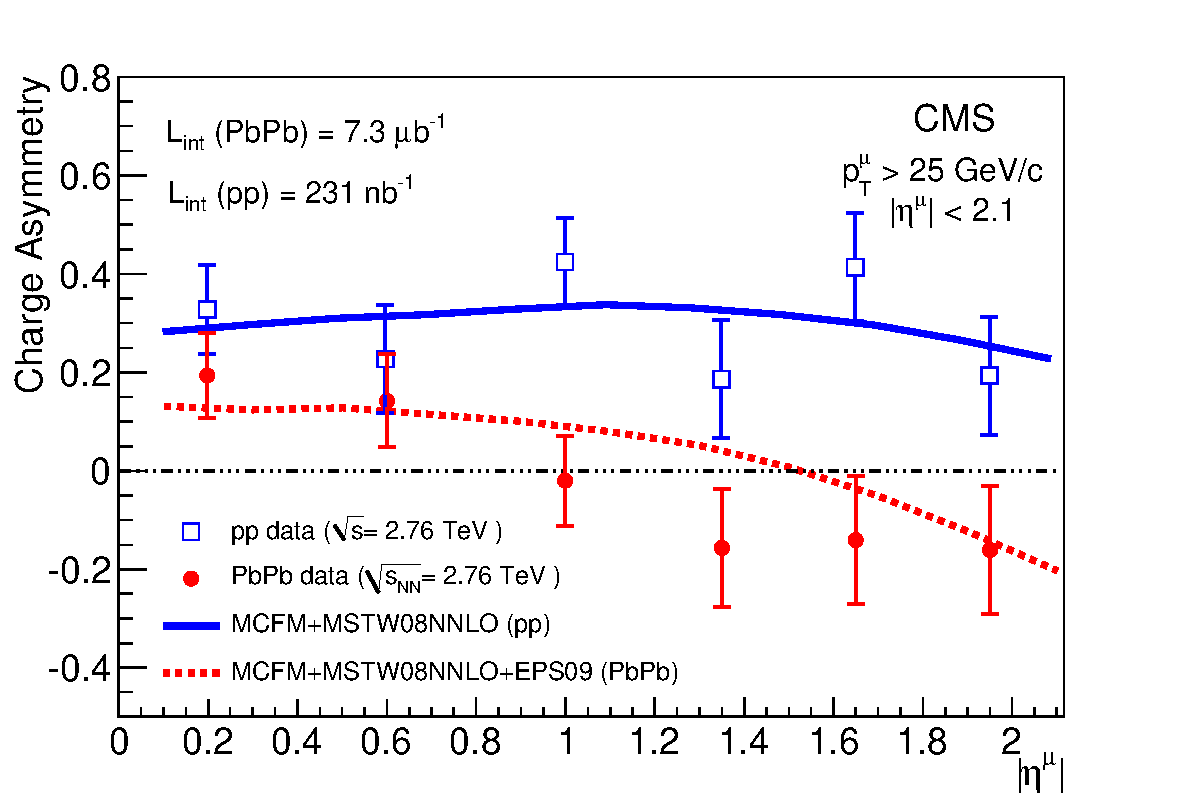
\includegraphics[width=0.49\textwidth]{electroweak_figs/Fig3.pdf}
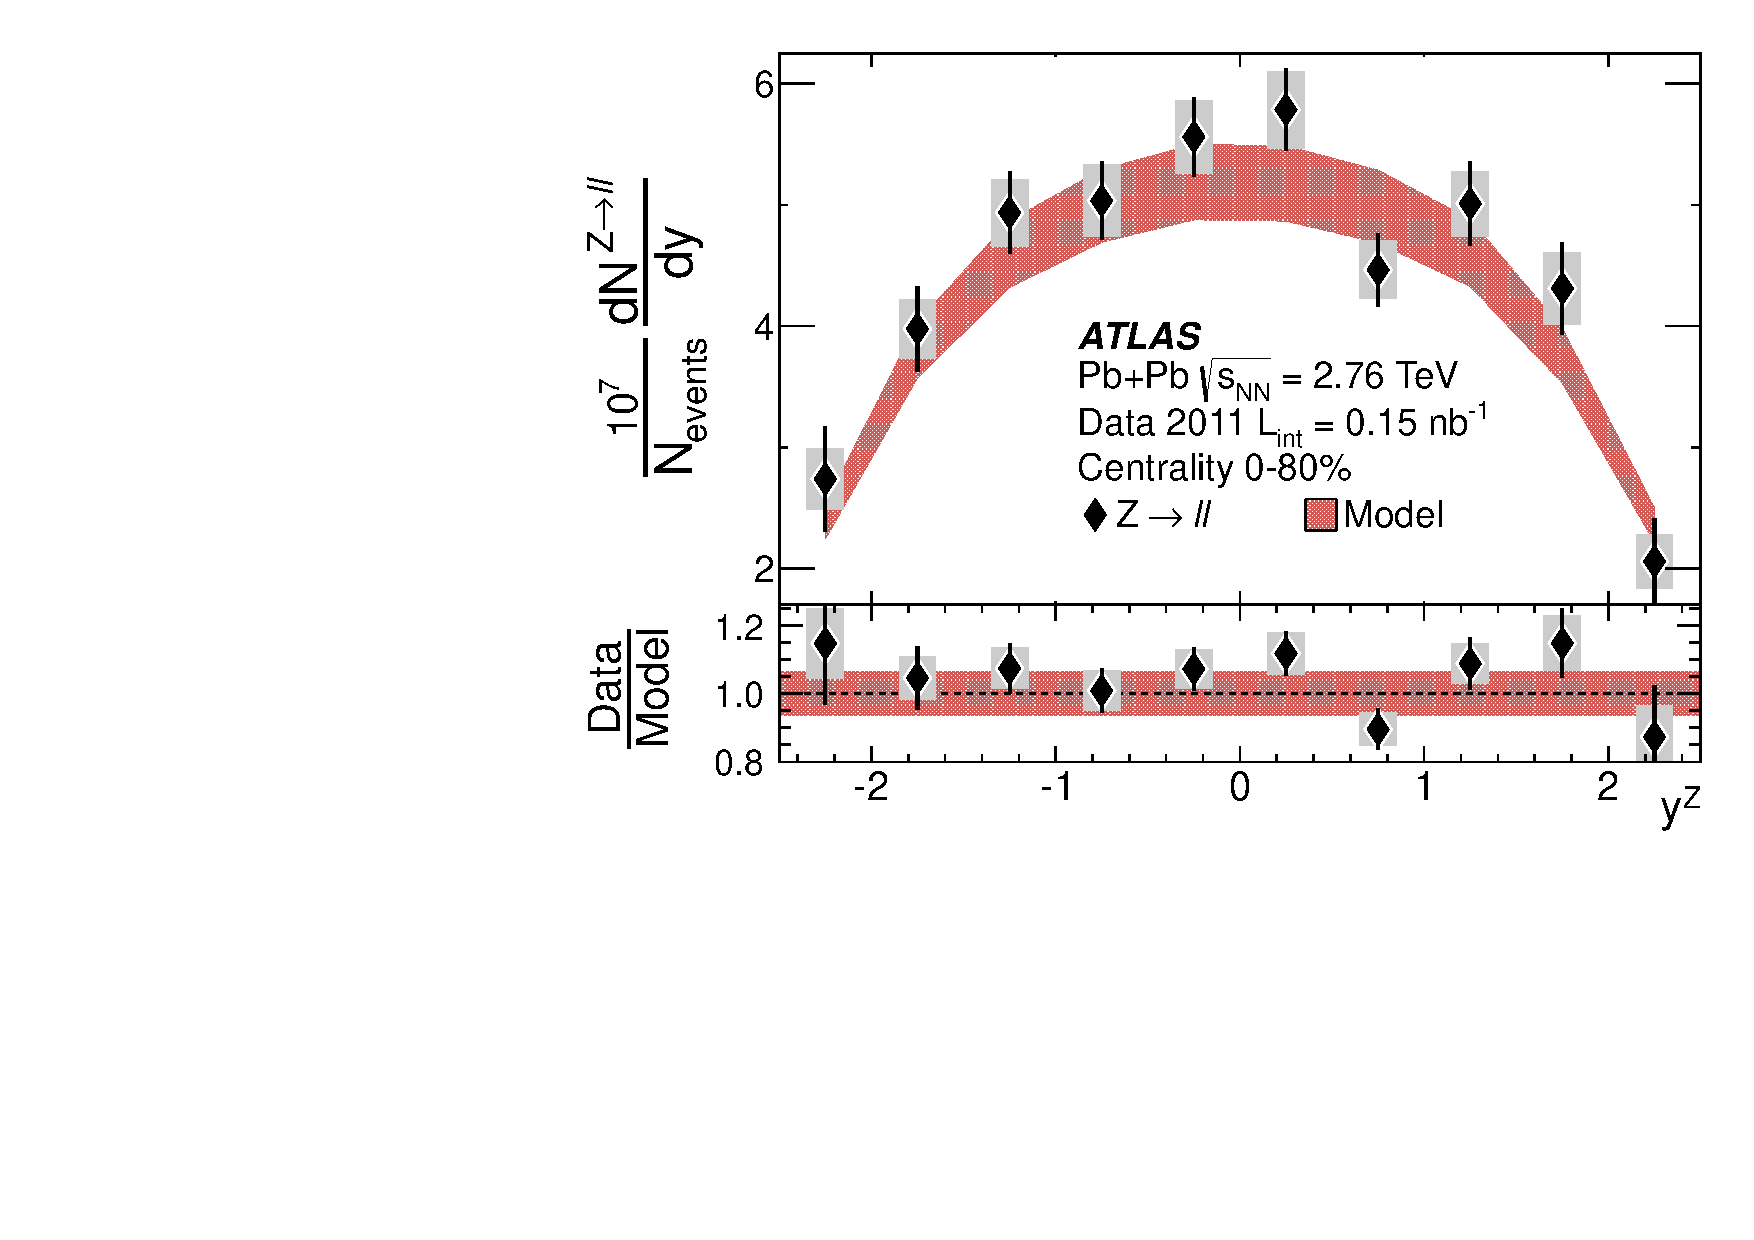
\includegraphics[width=0.45\textwidth]{electroweak_figs/fig_02.pdf}
\caption[]{(left) Charge asymmetry for W candidates, from CMS data~\cite{Chatrchyan:2012nt} (right) Rapidity dependence of $dN_{\mathrm{Z}}/dy$ compared to PYTHIA scaled to the NNLO cross section~\cite{Aad:2012ew}}
\label{fig:pas:zw_eta}
\end{center}
\end{figure}
Figure~\ref{fig:pas:zw_eta}(left) shows the pseudorapidity dependence of the charged lepton asymmetry for the muons associated with
W candidates ($A_\mu = (N_{\mathrm{W}^+}-N_{\mathrm{W}^-})/(N_{\mathrm{W}^+}+N_{\mathrm{W}^-})$), both for \PbPb and \pp data at the same CM energy
($\sqrt{s_\mathrm{NN}}=2.76$~TeV).  The evident differences between the \PbPb and \pp stem primarily from the neutrons in the
Pb nuclei, which modify the expected charge distribution, particularly in the forward direction where the Bjorken $x$ probed
is sensitive to the valence quarks.
Both data sets are compared with NNLO calculations of the W charge asymmetry and good agreement is found for both \pp and \PbPb.
While this suggests that no large nPDF effects are needed to accommodate the existing data, it was pointed out in Ref.~\cite{Paukkunen:2010qg}
that the scale factors in EPS09 formalism will cancel out in the charge asymmetry ratio, making this quantity suboptimal for
isolating nPDF modifications.

Figure~\ref{fig:pas:zw_eta}(right) shows the rapidity dependence of the per-event
Z boson yield in the 0-80\% centrality interval in \PbPb collisions
from the 2011 ATLAS \PbPb data.
The data is compared to the same distribution from PYTHIA (version 6.425), scaled to the NNLO total cross section,
and the appropriate mean nuclear thickness.
Good agreement is found between the heavy ion data and the absolutely-scaled PYTHIA reference, the ratio between them being consistent
with unity within the stated uncertainties.  While small effects at the 10-15\% level are not ruled out, nor are they required to
make sense of the current measurements.

\begin{figure}[t]
\begin{center}
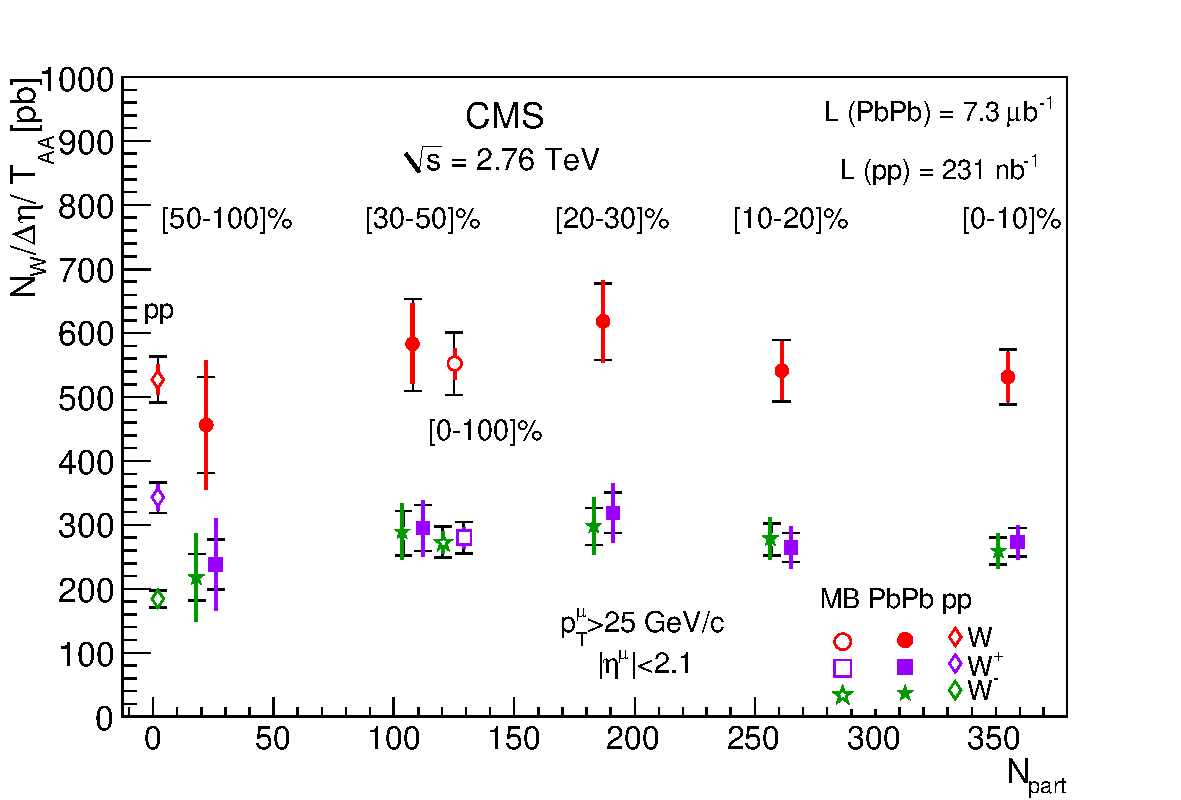
\includegraphics[width=0.54\textwidth]{electroweak_figs/Fig2.pdf}
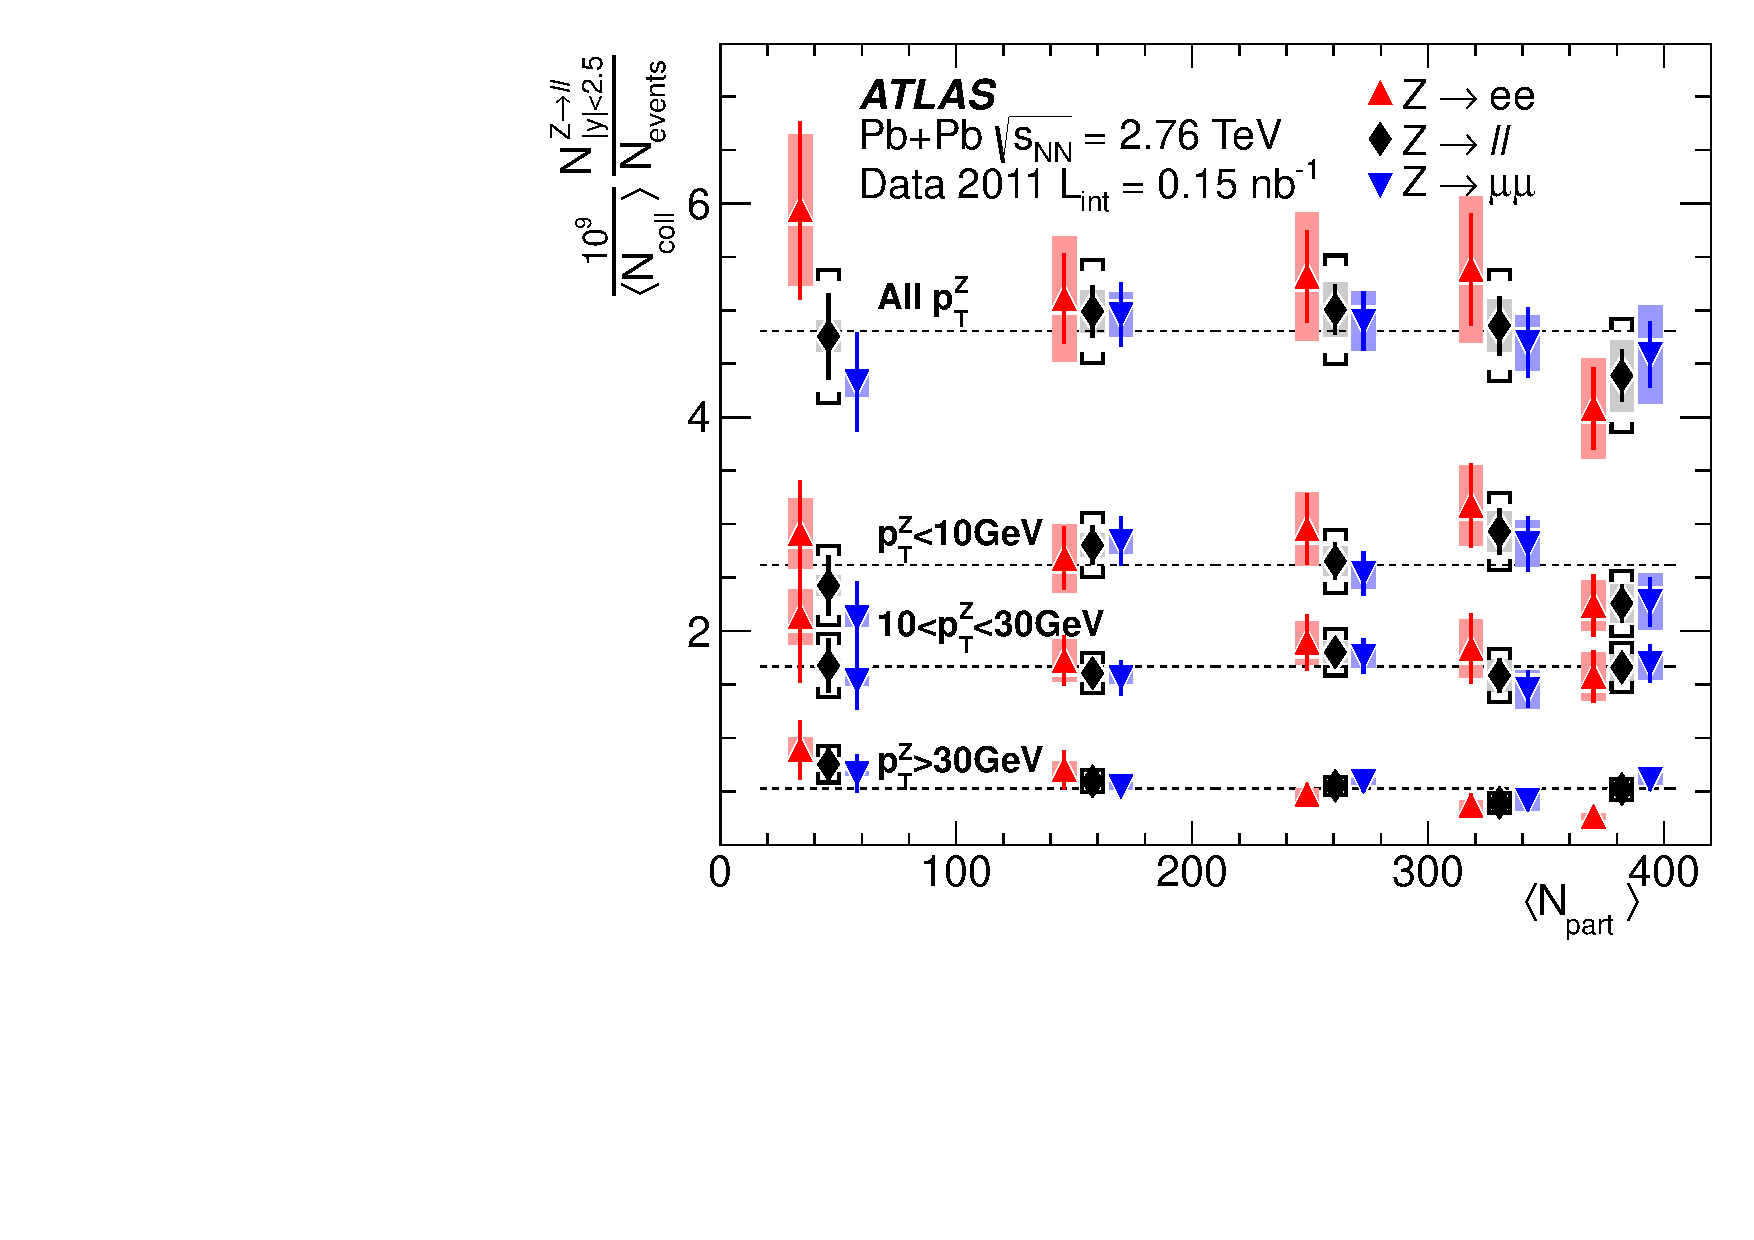
\includegraphics[width=0.44\textwidth]{electroweak_figs/fig_04.pdf}
\caption[]{(left) Yield per collision for W candidates, from CMS data~\cite{Chatrchyan:2012nt} (right) Yield per collision for Z's, in both electron and muon channels from ATLAS data~\cite{Aad:2012ew}.}
\label{fig:pas:zw_cent}
\end{center}
\end{figure}

The centrality dependence of the separate W charge states and the total from CMS
is shown in Figure~\ref{fig:pas:zw_cent}(left),
as a function of the number of participating nucleons, and for the \pp data.
While \pp shows a clear difference between positive and negative W's, reflecting the charges of the initial protons, there is little
difference between them in the \PbPb data, reflecting the additional down quarks introduced via the neutrons in the Pb nuclei.
The heavy ion data shows a clear scaling with centrality, once the W yields -- both for the charge-separated yields, and the
total -- are scaled by the number of binary collisions.
A similar message is found in the ATLAS Z data, shown in Figure~\ref{fig:pas:zw_cent}(right), which shows the Z yield, scaled by
the number of binary collisions, also as a function of the number of the mean number of participating nucleons for each
centrality interval.  The ATLAS data also shows that the centrality dependence is the same for the dielectron and dimuon channels,
and even for selected intervals in the Z \pT.

\subsection{Measurement of isolated photons in \PbPb collisions}

\begin{figure}[!htb]
\begin{center}
\raisebox{5mm}{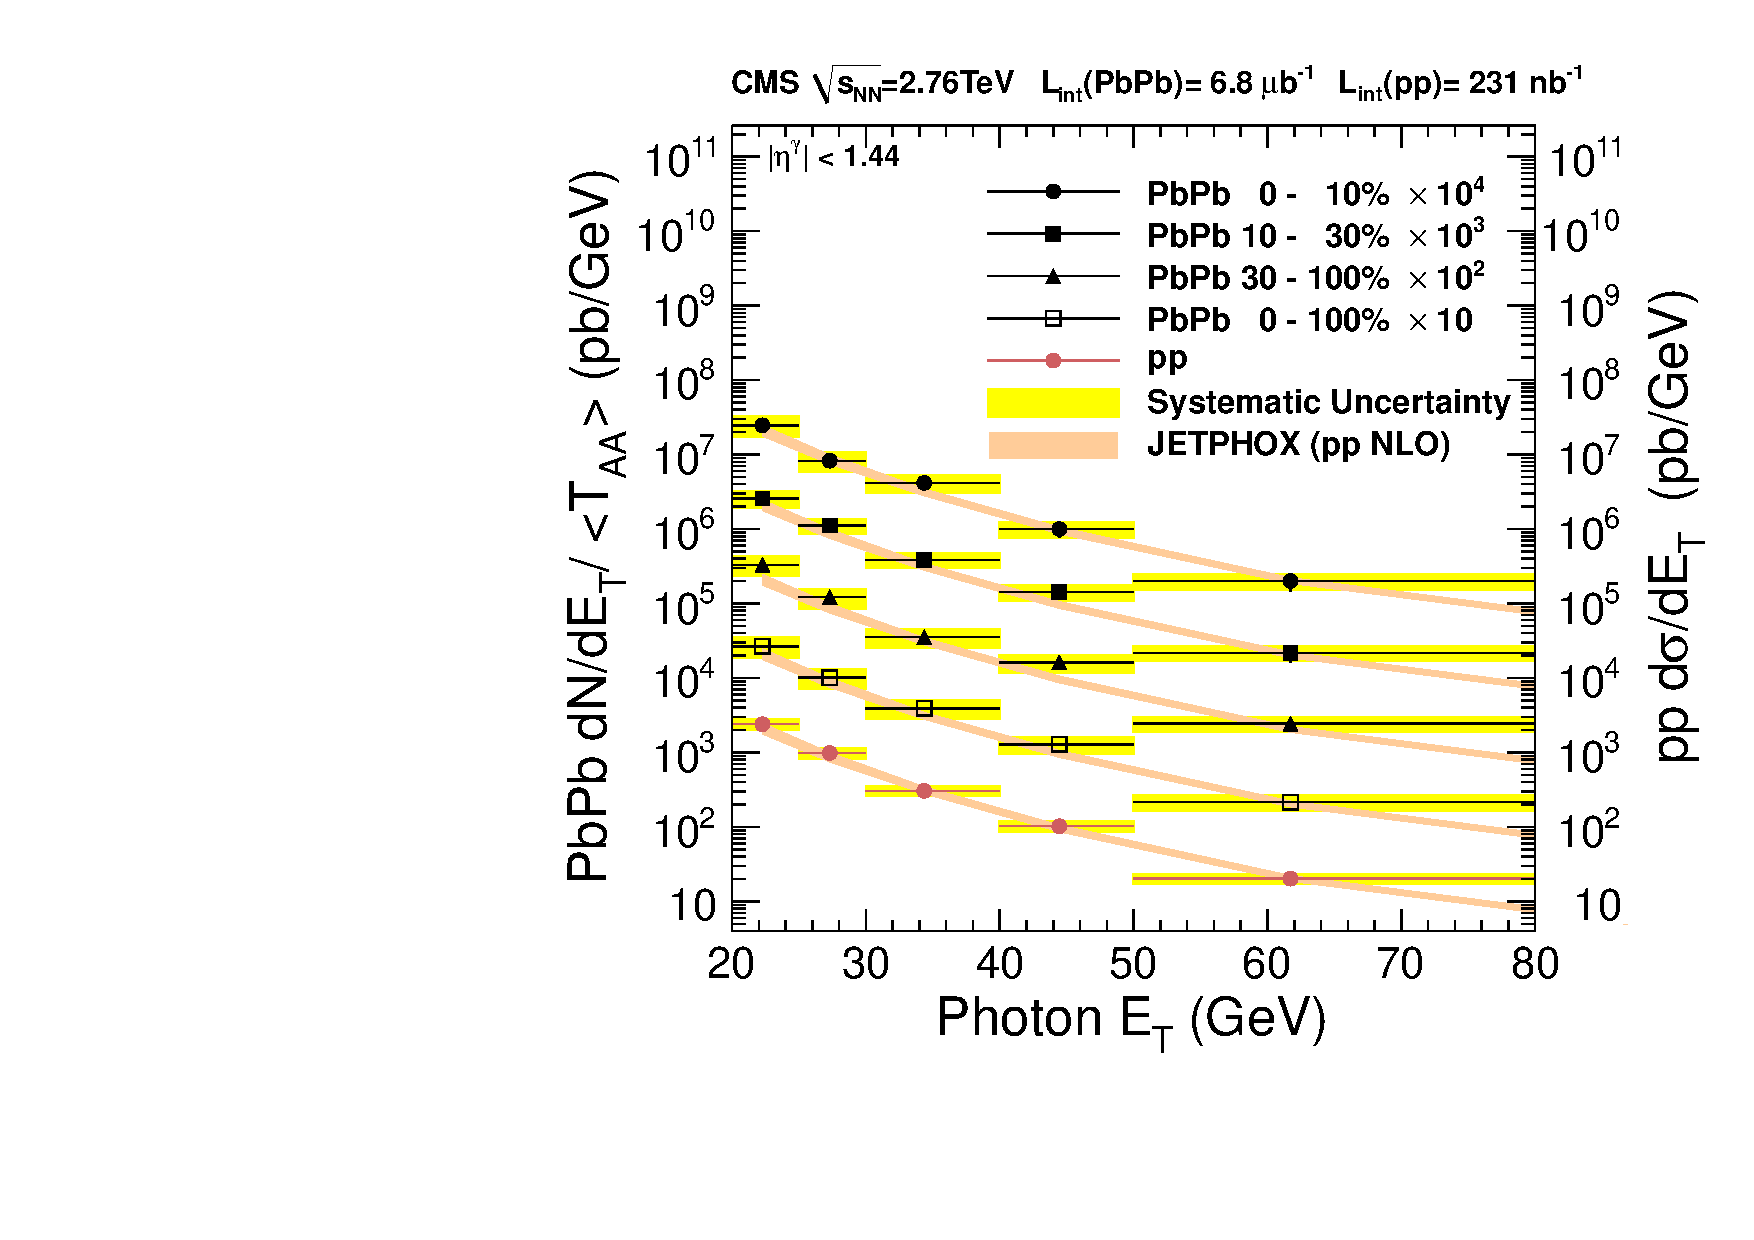
\includegraphics[width=0.50\textwidth]{electroweak_figs/TAAScaling.pdf}}
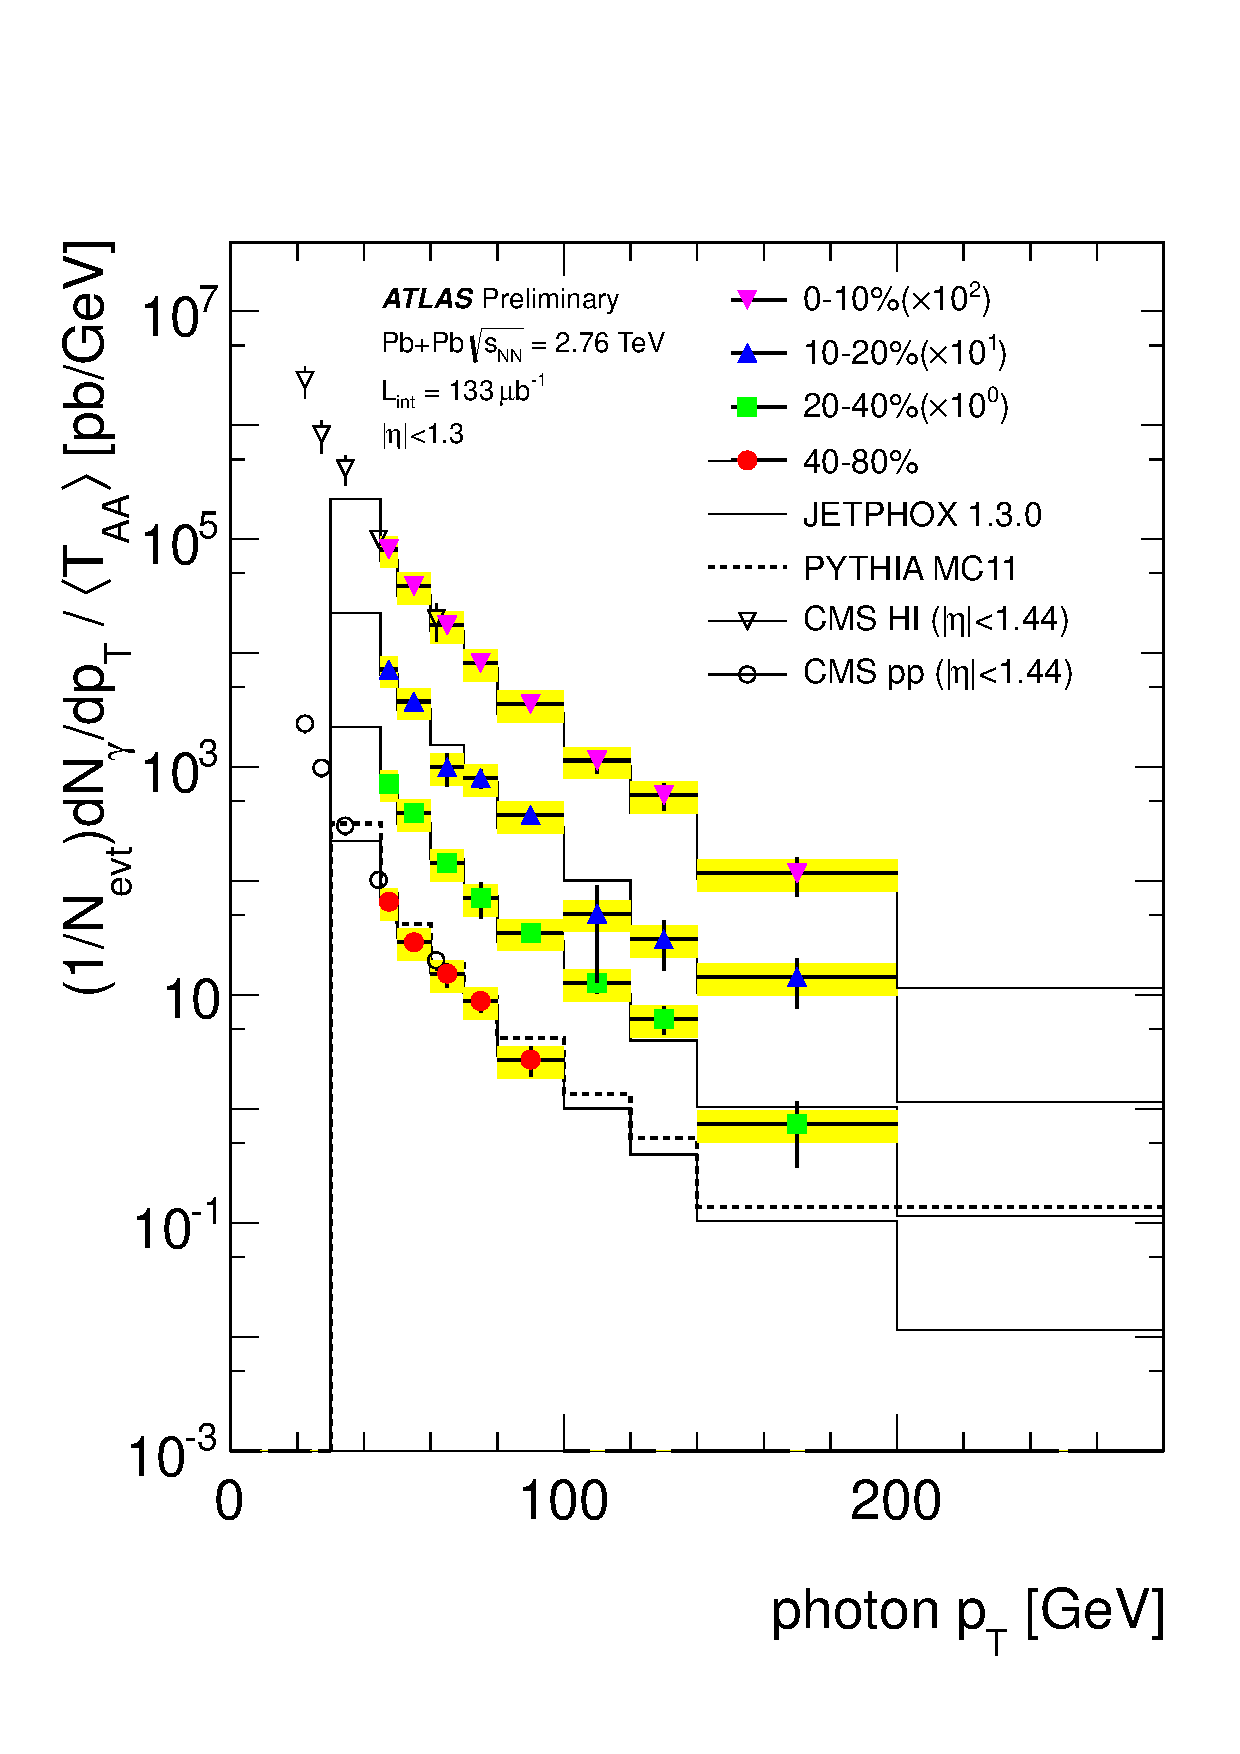
\includegraphics[width=0.40\textwidth]{electroweak_figs/ph_fig_11.pdf}
\caption[]{(left) Photon yields scaled by the mean nuclear thickness function for $|\eta|<1.44$, from CMS data~\cite{Chatrchyan:2012vq} (right) The similar quantity from ATLAS, for $|\eta|<1.3$, from ATLAS data~\cite{ATLAS:2012zla}.}
\label{fig:pas:photon}
\end{center}
\end{figure}

The measurement of photons in heavy ion collisions is also an important contribution to the
study of the \PbPb initial state, with some advantages and disadvantages.  Unlike Z and W bosons,
no energy from the initial 2-to-2 scattering process is used in the boson mass,
and so the cross sections at high \pT\ are substantially higher at the same transverse momentum.
However, photon measurements do not provide a clear mass peak, and nor are they associated with
a track measured in an inner tracker.  This means that backgrounds are an irreducible part of
the measurement, particularly at low \pT, where one expects large contribution from jet fragmentation
into high momentum neutral pions or eta mesons.

At low \pT, ALICE has performed a preliminary measurement of the spectrum of direct photons
using the so-called ``subtraction'' method~\cite{Wilde:2012wc}.
In this approach, inclusive photons are measured,
and the contribution from hadron decays is estimated through a combination of direct measurements
and a cocktail based on $m_{\rm T}$-scaling.
Using this, the remaining contribution from direct photons is extracted and compared to
perturbative QCD calculations.  This has been performed on 7~TeV \pp data, and good agreement
with pQCD is found.  In the 0--40\,\% centrality interval in \PbPb, good agreement is found above
$\pT=4$~GeV with a scaled NLO calculation at the \PbPb CM energy.  However, an excess is observed
below 4~GeV, which is fit by an exponential and gives an inverse slope parameter of
$T_{\mathrm{LHC}} = 304 \pm 51^{\mathrm{syst+stat}}$ MeV.  By comparison to a similar
measurement from PHENIX, which observes an inverse slope of
$T_{\mathrm{PHENIX}}=221 \pm 19^{\mathrm{stat}} \pm 19^{\mathrm{syst}}$ MeV for the 0-20\%
centrality interval at the top RHIC energy~\cite{Adare:2008ab},
ALICE concludes that the initial temperature at the LHC is higher
than that measured at RHIC.

At high \pT, two primary techniques are used to increase the purity of the photon sample, which is typically
$O(0.1\%)$ based on the expected relative yields of photons and jets.  The first is to select
photon candidates as electromagnetic clusters which pass a set of selection criteria, trained on
photon simulations to efficiently reject electromagnetic decays while keeping most of the
produced photons.  These criteria involve both the ``shape'' of the cluster (since photon showers
are typically quite narrow), as well as the presence of energy in the ``hadronic'' section of the
experimental calorimeters (since photon showers should typically be well-contained in the front
electromagnetic sections).
The second technique is to require that the photon candidate is ``isolated'', i.e. only a limited
amount of ambient energy, including both electromagnetic and hadronic contributions,
is allowed to be present near the photon.  In the context of a heavy ion collision, where there
is typically a substantial amount of uncorrelated energy present, techniques must be applied to
estimate and remove this energy event by event.  However, even after doing this, one must account
for real photons with an upward fluctuation of ambient energy nearby (``leakage'') as well
as fake photons with a downward fluctuation, passing the nominal selection criteria.
Thus, shower-shape discriminators are typically combined with an isolation requirement, and various
means exist to combine this information to estimate the true purity of a photon sample in a
data-driven fashion.

The CMS photon measurement is performed using electromagnetic clusters in the CMS ECAL, with the
CMS tracks and HCAL used to tag backgrounds from electrons or hadronic decays.
The signal from prompt isolated photons is extracted using a two-component template fit to
the distribution of $\sigma_{\eta\eta}$, a variable which reflects the width of the cluster
in the $\eta$ direction.  The signal is derived from PYTHIA $\gamma$+jet events, embedded
into real \PbPb data events.  The background distribution is derived from a set of photon
candidates which are required to fail the isolation selection.
After subtracting the extracted backgrounds and correcting for efficiency and resolution
effects, the yield of photons is presented as a function of \pT in three centrality intervals
as well as a minimum-bias (0-100\%) interval.  A similar analysis performed on pp data is
also shown.
In Figure~\ref{fig:pas:photon}(left),
both the heavy ion and pp data are compared with an NLO pQCD calculation (using the
JETPHOX package) by scaling the calculation by the mean nuclear
thickness function $\langle T_{\mathrm{AA}} \rangle$ relevant for each interval.
It is found that the NLO calculations agree with the pp and heavy ion data in all cases, within
the stated statistical and systematic uncertainties.  This demonstrates that, like the
Z and W results, the photon yields scale with the number of binary collisions.
However, while the Z and W results focused on integrated yields, the photons show that
there is also no modification of the spectral shape.

ATLAS performed a similar analysis, using the ``double sideband'' technique to estimate the
photon fraction in each \pT and centrality interval for $|\eta|<1.3$.
In Figure~\ref{fig:pas:photon}(right), the preliminary ATLAS data is shown compared with both
the CMS data and JETPHOX 1.3.0 results.  The ATLAS and CMS data agree well (given the 5\%
difference in the $\eta$ range) and ATLAS data agree with JETPHOX out to $\pT = 200$~GeV.

